\documentclass[10pt,hyperref={CJKbookmarks=true},xcolor=dvipsnames,aspectratio=169]{beamer}
\usetheme[navigation]{UMONS}
\usepackage[utf8]{inputenc}
\usepackage{verbatim}
\usepackage{ctex}

\title[Predicting ARBs]{Predicting aging-related bugs using software complexity metrics}
\author[B.Jason]{Jason \textsc{Bury}}
\institute[]{%
 Faculté des Sciences\\
  Université de Mons
  \\[2ex]
  
\includegraphics[height=4ex]{figures/UMONS}\hspace{2em}%
  \raisebox{-1ex}{
\includegraphics[height=6ex]{figures/UMONS_FS}}
}

\begin{document}
\maketitle
\section{Introduction}
\subsection{Aging-related bugs}

\begin{frame}
 \frametitle{Aging-Related Bugs}
 \framesubtitle{Mandelbug}
 If
 \begin{itemize}
  \item A time lag between the fault activation and the failure occurence.
  \item Bug influenced by timing of operations or order of operations or environment interactions.
 \end{itemize}
 \vspace{1cm}
 \begin{tabular}{llll}
  Then & $\Longrightarrow$ & \emph{Mandelbug} & :-( \\
  Else & $\Longrightarrow$ & \emph{Bohrbugs} & :-) , can thus be easily isolated
 \end{tabular}
\end{frame}

\begin{frame}
 \frametitle{Aging-Related Bugs试试中文}
 \framesubtitle{Aging-related mandelbug}
 If Mandelbug and\\
 \vspace{1cm}
 The bug causes the accumulation of internal error states
 \begin{center}
  \large Or \normalsize
 \end{center}
 The running time increase the risk of the bug activation/propagation\\
 \vspace{1cm}
 Then $\Longrightarrow$ \emph{Aging-related Mandelbug} :'( \\
 \small Also called \emph{Aging-related bug} or \alert{ARB}.\normalsize
\end{frame}

\begin{frame}
 \frametitle{Aging-Related Bugs}
 \framesubtitle{Examples}
 \begin{exampleblock}{What can causes an ARB ?}
  \begin{itemize}
   \item Numerical error due to rounding or imprecision accrue over time
   \item A malloc() without free()
   \item A queue continuously increased
   \item Size of ressource exceeded
   \item ...
  \end{itemize}
 \end{exampleblock}
\end{frame}

\subsection{How to detect}
\begin{frame}
 \frametitle{How can we detect them ?}
 short answer: \alert{Select metrics then use a classifier !}\\
 But, there are remaining questions about that solution:\\
 \begin{block}{Questions}
  \begin{itemize}
   \item Which metrics to use ?
   \item New metrics ?
   \item Which classifier to use ?
   \item will be the classifier effective for all projects ?
  \end{itemize}
 \end{block}
\end{frame}

\begin{frame}
 \frametitle{Project used as training set}
 3 complex projects will be used.\\
 \begin{itemize}
  \item Linux
  \item MySQL
  \item CARDAMOM, a middleware for air traffic control systems
 \end{itemize}
 \vspace{0.2cm}
 ARBs are found manually.\\
\end{frame}
% middleware: un réseau d'échange d'informations entre différentes applications informatiques.

\section{Classifiers}

\subsection{Metrics to use}
\begin{frame}
 \frametitle{Which metrics to use ?}
 46 metrics correlated with bug density:
 \begin{itemize}
  \item Program size. 26 metrics\\
  (lines of codes, comments, blank, semicolons, functions, preprocessor)
  \item Cyclomatic complexity. 11 metrics
  \item Halstead metrics. 9 metrics
 \end{itemize}
\end{frame}
% TODO liste complete en annexe
% Program size: cout lines of code, blank lines, comments, functions, classes, semicolons.
% Program size: count, average, ration, etc,

\begin{frame}
 \frametitle{Halstead metrics}
 Halstead metrics: set of metrics based on the number of operands and number of operators.\\
 Based on
 \begin{center}
  \begin{tabular}{ll}
   $\eta_1$ & = The number of distinct operators\\
   $\eta_2$ & = The number of distinct operands\\
   $N_1$ & = The total number of operators\\
   $N_2$ & = The total number of operands\\
  \end{tabular}
 \end{center}
 \begin{exampleblock}{Some halstead metrics}
  \begin{itemize}
   \item Program vocabulary = $\eta = \eta_1 + \eta_2$
   \item Program length = $N = N_1 + N_2$
   \item Volume = $N \times \text{log}_2\eta$
   \item Difficulty = $\frac{\eta_1}{2} \times \frac{N_2}{\eta_2}$
  \end{itemize}
 \end{exampleblock}
\end{frame}

\subsection{Results without new metrics}
\begin{frame}
 \frametitle{Tried classifiers}
 \begin{itemize}
  \item Naive Bayes (NB)
  \item Bayesian networks (BayesNet)
  \item Decision trees (DecTree)
  \item Logistic regression (Logistic)
 \end{itemize}
\end{frame}
%TODO montrer la gueule que ça a

\begin{frame}
 \frametitle{Results without new metrics}
 \framesubtitle{Terminology}
 $$PD = \text{Probability of detection} = \frac{\text{true positives}}{\text{true positives + false negatives}} . 100\%$$
 \vspace{0.1cm}
 $$PF = \text{Probability of false alarms} = \frac{\text{false positives}}{\text{true negatives + false positives}} . 100\%$$
 \vspace{0.1cm}
 $$Bal = Balance = 100 - \frac{\sqrt{(0-PF)^2 + (100-PD)^2}}{\sqrt{2}}$$
 \begin{center}
  \begin{tabular}{ll}
   log : & metrics at a logarithmic scale
  \end{tabular}
 \end{center}
 \small note: the difference between the highest and the second highest value can be statistically not significant. See numbers in bold. \normalsize
\end{frame}
%Probability of detection is the probability that a ARB-prone module will be classified as ARB-prone
%Probability of false alamrs is the probability that a non-ARB-prone module is erroneously identified as ARB-prone
%A classifier with a high PD can also have a high PF (imagine a classifier that always answer 'yes') So balance is a trade-off

\begin{frame}
 \frametitle{Results without new metrics}
 \framesubtitle{Linux}
 \begin{center}
 \begin{tabular}{lrrr}
  \hspace{0.2cm} Classifier & PD & PF & Bal\\
  \hline
  NB & 60.13 & 12.46 & \textbf{69.24}\\
  NB + log &  \textbf{92.33} & \textbf{37.09} & \textbf{72.28}\\
  BayesNet & 3.72 & 1.85 & 31.91\\
  BayesNet + log & 5.34 & 1.95 & 33.06\\
  DectTree & 0.00 & 0.03 & 29.30\\
  DectTree + log & 0.00 & 0.00 & 29.30\\
  Logistic & 1.00 & 0.63 & 30.01\\
  Logistic + log & 3.84 & 0.62 & 32.01\\
  \hline
 \end{tabular}
 \end{center}
\end{frame}

\begin{frame}
 \frametitle{Results without new metrics}
 \framesubtitle{MySQL}
 \begin{center}
 \begin{tabular}{lrrr}
  \hspace{0.2cm} Classifier & PD & PF & Bal\\
  \hline
  NB & 49.14 & 10.46 & 63.02\\
  NB + log &  \textbf{88.30} & \textbf{34.67} & \textbf{73.53}\\
  BayesNet & 44.57 & 8.65 & 60.26\\
  BayesNet + log & 44.50 & 8.65 & 60.21\\
  DectTree & 11.21 & 2.64 & 37.17\\
  DectTree + log & 11.28 & 2.65 & 37.22\\
  Logistic & 22.93 & 4.46 & 45.40\\
  Logistic + log & 25.07 & 5.13 & 46.88\\
  \hline
 \end{tabular}
 \end{center}
\end{frame}

\begin{frame}
 \frametitle{Results without new metrics}
 \framesubtitle{CARDAMOM}
 \begin{center}
 \begin{tabular}{lrrr}
  \hspace{0.2cm} Classifier & PD & PF & Bal\\
  \hline
  NB & 0.00 & 7.18 & 29.08\\
  NB + log &  \textbf{54.50} & \textbf{25.15} & \textbf{53.25}\\
  BayesNet & 0.00 & 0.00 & 29.30\\
  BayesNet + log & 0.00 & 0.00 & 29.30\\
  DectTree & 0.00 & 0.00 & 29.30\\
  DectTree + log & 0.00 & 0.00 & 29.30\\
  Logistic & 0.00 & 1.21 & 29.30\\
  Logistic + log & 0.00 & 0.65 & 29.30\\
  \hline
 \end{tabular}
 \end{center}
\end{frame}

\begin{frame}
 \frametitle{Results without new metrics}
 \begin{center}
  $\Longrightarrow$ \alert{Select the Naive Bayes classifier with metrics at a logarithmic scale.}
 \end{center}
 \vspace{1cm}
 High probability of detection but high probability of false alarm.
 Still useful for Verification \& Validation process:
 \begin{center}
  \alert{avoids to inspect the files classified as non-ARB !}
 \end{center}
\end{frame}

\section{Attribute selection}
\subsection{Impact}

\begin{frame}
 \frametitle{Attribute selection}
 \begin{center}
  \alert{Which attribute to select ?}
 \end{center}
 For each project, sort metrics by \emph{Information Gain}:\\
 \vspace{0.2cm}
 \begin{tabular}{ll}
  $InfoGain(A_i)$ = & the number of bits of information obtained\\
   & by knowing the value of attribute $A_i$
 \end{tabular}
 \\
 \vspace{0.4cm}
 Then, in a decreasing order of $InfoGain(A_i)$, compute PD, PF and Bal with the NB+log classifier.
\end{frame}
%discarding a redundant metric could improve performance

\begin{frame}
 \frametitle{Impact of attribute selection}
 \framesubtitle{Linux}
 \begin{center}
  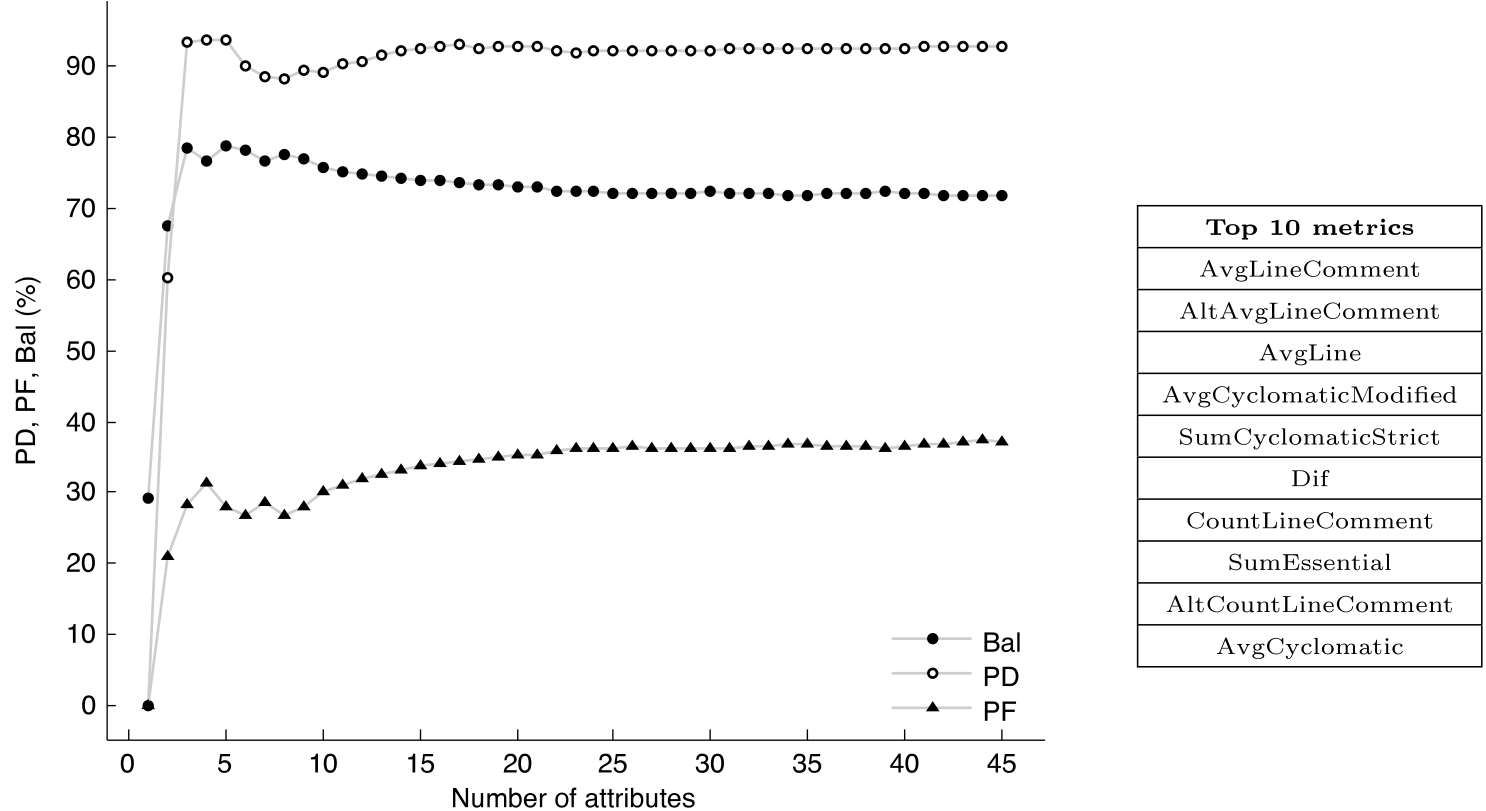
\includegraphics[width=\textwidth]{figures/attributesLinux.png}
 \end{center}
\end{frame}

\begin{frame}
 \frametitle{Impact of attribute selection}
 \framesubtitle{MySQL}
 \begin{center}
  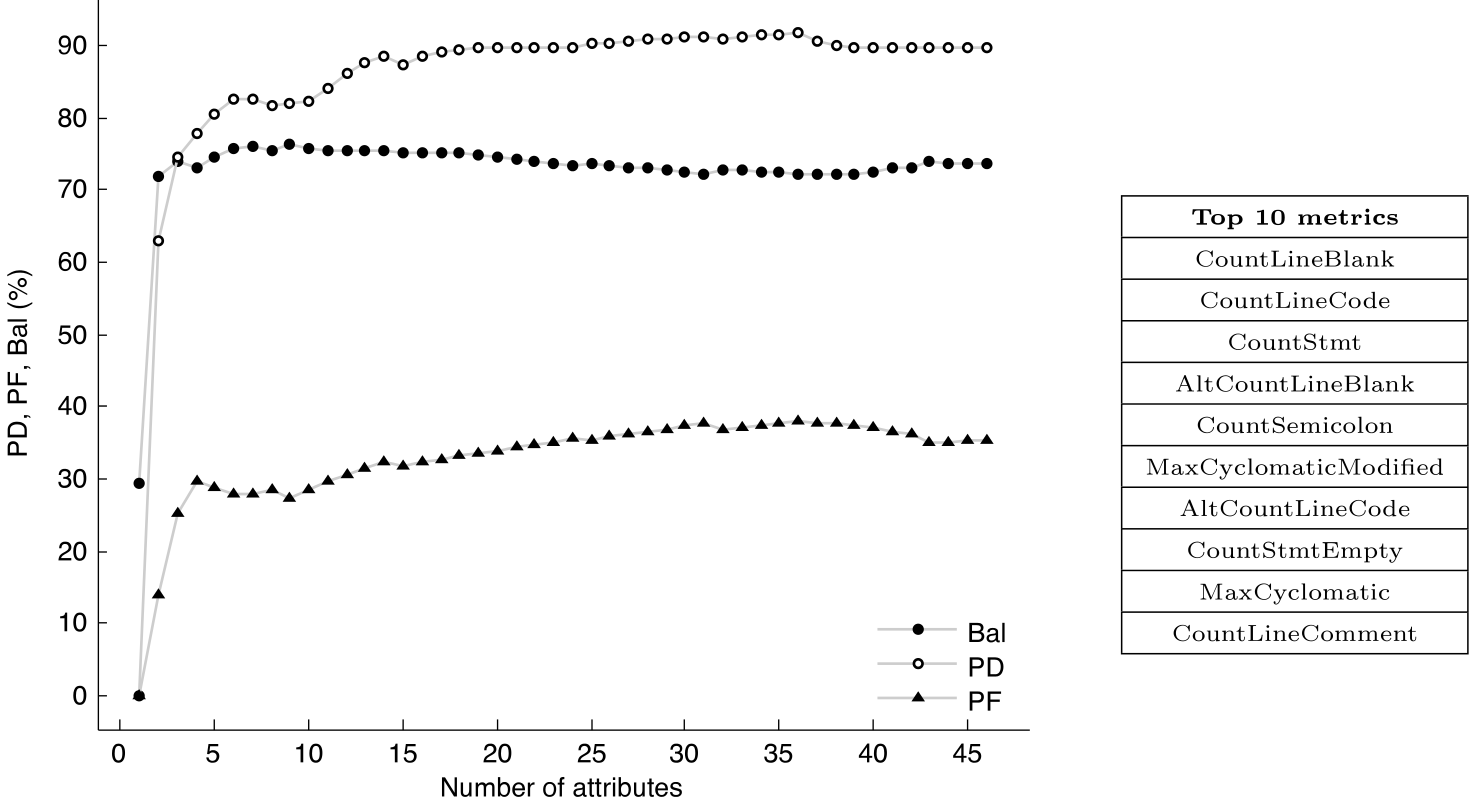
\includegraphics[width=\textwidth]{figures/attributesMysql.png}
 \end{center}
\end{frame}

\begin{frame}
 \frametitle{Impact of attribute selection}
 \framesubtitle{CARDAMOM}
 \begin{center}
  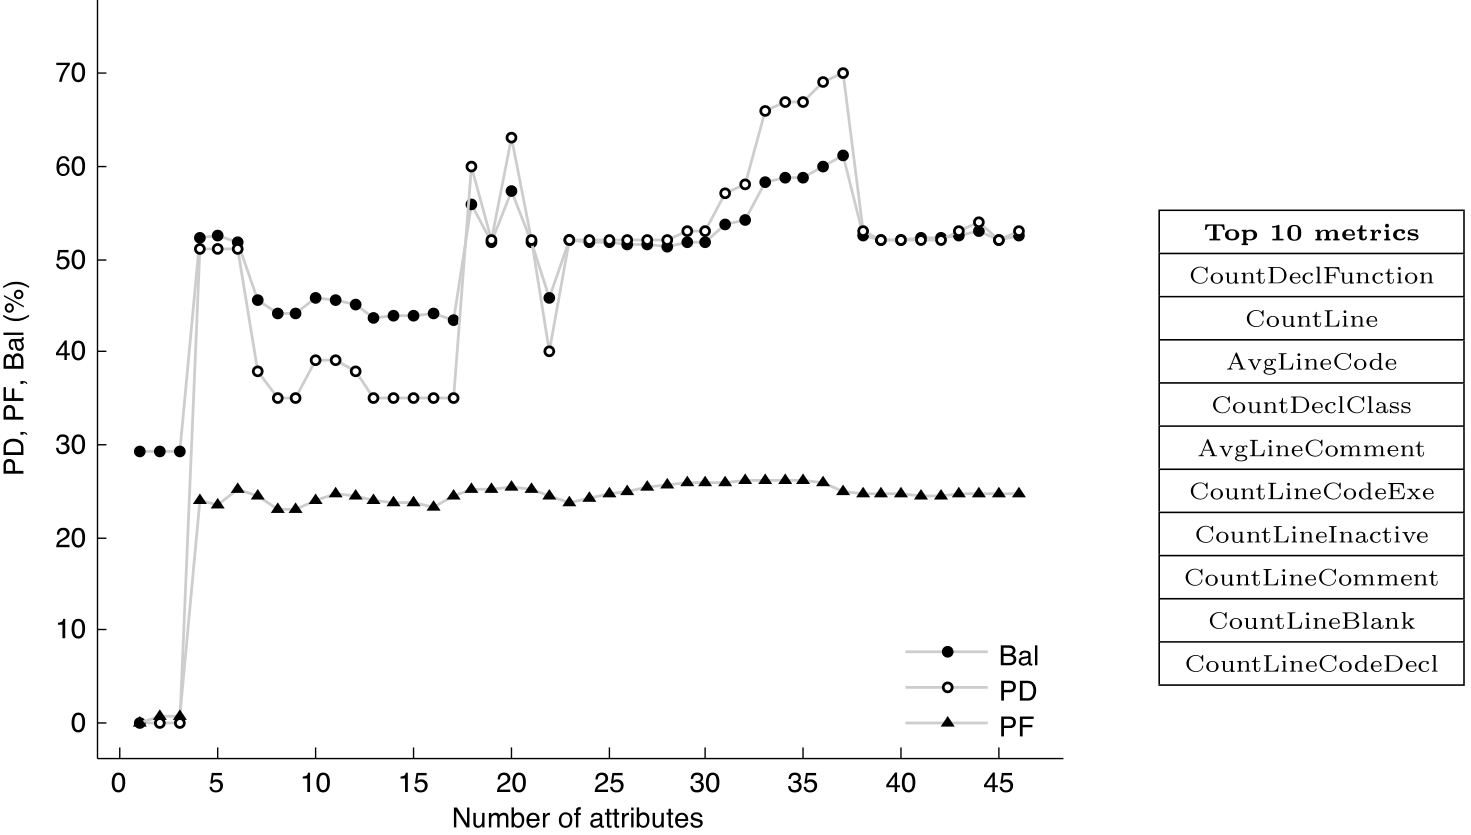
\includegraphics[width=\textwidth]{figures/attributesCardamom.png}
 \end{center}
\end{frame}

\begin{frame}
 \frametitle{Impact of attribute selection}
 \begin{itemize}
  \item Top metrics not the same
  \item Need about 5 top metrics
  \item With all metrics, nearly the same results than with 5
 \end{itemize}
 \vspace{0.5cm}
 \begin{center}
  $\Longrightarrow$ \alert{We keep the full set of metrics.}
 \end{center}
\end{frame}

\section{New metrics}

\subsection{New metrics}
\begin{frame}
 \frametitle{New metrics}
 \begin{center}
  \alert{lot of ARB are about memory leaks.}
 \end{center}
 6 new metrics related to memory usage, the \alert{ARMs}:
 \vfill
 \begin{itemize}
  \item \emph{AllocOps} : Number of instruction about allocation of memory
   \begin{center}
    (malloc)
   \end{center}
  \item \emph{DeallocOps} : Number of instruction about Deallocation of memory
   \begin{center}
    (free)
   \end{center}
 \end{itemize}
\end{frame}
% We introduce metrics related to memory usage because we noticed that lot of ARB are about memory leaks

\begin{frame}[fragile]
 \frametitle{New metrics}
 \begin{itemize}
  \item \emph{DerefUse} : Number of times a pointer variable is dereferenced to write
   \begin{exampleblock}{Dereferencing a structure member}
    \begin{verbatim}typedef struct X { int a; int b; } X;
X x;
X* p = &x;
p->a = 3.14159;\end{verbatim}
   \end{exampleblock}
  \item \emph{DerefSet} : Number of times a pointer variable is dereferenced to read
   \begin{exampleblock}{Dereferencing \texttt{p} and read}
    \begin{verbatim}printf("%d", p->a);\end{verbatim}
   \end{exampleblock}
 \end{itemize}
\end{frame}

\begin{frame}
 \frametitle{New metrics}
 \begin{itemize}
  \item \emph{UniqueDerefSet} : Same as DerefSet but variable counted one time per file
  \item \emph{UniqueDerefUse} : Same as DerefUse but variable counted one time per file
 \end{itemize}
 \vfill
\end{frame}

\subsection{Results}
\begin{frame}
 \frametitle{Results with new metrics}
 \framesubtitle{Linux}
 \begin{center}
 \begin{tabular}{lrrr}
  \hspace{0.2cm} Classifier & PD & PF & Bal\\
  \hline
  NB & 60.13 & 12.46 & 69.24\\
  NB + log &  \textbf{92.33} & \textbf{37.09} & 72.28\\
  NB + ARMs & 58.13 & 11.88 & 68.34\\
  NB + log + ARMs & \textbf{93.56} & 35.90 & \textbf{73.25}\\
  \hline
 \end{tabular}
 \end{center}
 \vspace{0.5cm}
 It decreases PF.
\end{frame}

\begin{frame}
 \frametitle{Results with new metrics}
 \framesubtitle{MySQL}
 \begin{center}
 \begin{tabular}{lrrr}
  \hspace{0.2cm} Classifier & PD & PF & Bal\\
  \hline
  NB & 49.14 & 10.46 & 63.02\\
  NB + log &  \textbf{88.30} & \textbf{34.67} & 73.53\\
  NB + ARMs & 48.42 & 10.06 & 62.61\\
  NB + log + ARMs & \textbf{88.37} & 32.99 & \textbf{74.69}\\
  \hline
 \end{tabular}
 \end{center}
 \vspace{0.5cm}
 It decreases PF.
\end{frame}

\begin{frame}
 \frametitle{Results with new metrics}
 \framesubtitle{CARDAMOM}
 \begin{center}
 \begin{tabular}{lrrr}
  \hspace{0.2cm} Classifier & PD & PF & Bal\\
  \hline
  NB & 0.00 & 7.18 & 29.08\\
  NB + log & 54.50 & \textbf{25.15} & 53.25\\
  NB + ARMs & 0.00 & 6.57 & 29.12\\
  NB + log + ARMs & \textbf{68.00} & 10.22 & \textbf{70.32}\\
  \hline
 \end{tabular}
 \end{center}
 \vspace{0.5cm}
 It decreases PF and increases PD. $\Longrightarrow$ \alert{We keep ARMs.}
\end{frame}


\section{cross classification}

\subsection{cross-component}
\begin{frame}
 \frametitle{Cross-component classification}
 \alert{In the same project, Can we predict ARB in a new component ?}\\
 Results of classifier when we exclude a component and use it as a test set:
 \begin{center}
  \begin{tabular}{l l|r r r}
   Project & Component & PD & PF & Bal\\
   \hline
   Linux & Network drivers & 88.9 & 41.7 & 69.5\\
    & SCSI drivers & 75.0 & 27.6 & 73.7\\
    & EXT3 & 100.0 & 52.2 & 63.1\\
    & IPv4 & 100.0 & 52.2 & 63.1\\
   \hline
   MySQL & InnoDB & 65.6 & 16.5 & 73.0\\
    & Replication & 100.0 & 28.6 & 79.8\\
    & Optimizer & 100.0 & 69.7 & 50.7\\
   \hline
   CARDAMOM & Foundation & 0.0 & 0.0 & 29.3\\
    & Load Balancing & 100.0 & 9.0 & 93.7\\
   \hline
  \end{tabular}
 \end{center}
 \small (0\% of ARB detected in Foundation because there is only one ARB.) \normalsize
\end{frame}
%SCSI = Small Computer System Interface. Bus connecting the computer to peripherics or computers

\subsection{cross-project}
\begin{frame}
 \frametitle{Cross-project classification}
 \alert{Can those classifiers predict ARB for another project ?}\\
 Results of classifier when the training set comes from another project than the test set:
 \begin{center}
 \begin{tabular}{l|r r r|r r r|r r r}
  Train & \multicolumn{3}{c}{Linux} & \multicolumn{3}{c}{MySQL} & \multicolumn{3}{c}{CARDAMOM}\\
  ~ & PD & PF & Bal & PD & PF & Bal & PD & PF & Bal\\
  \hline
  Linux & - & - & - & 82.9 & 23.8 & 79.3 & 0.0 & 0.2 & 29.3\\
  MySQL & 100.0 & 50.7 & 64.2 & - & - & - & 33.3 & 11.8 & 52.1\\
  CARDA & 0.0 & 0.1 & 29.3 & 0.0 & 0.6 & 29.3 & - & - & -\\
  \hline
 \end{tabular}
 \end{center}
 Low performance with CARDAMOM due to the difference of caracteristics between CARDAMOM and the two others.
 \begin{center}
  (CARDAMOM in pure C++, MySQL in mixed C/C++, Linux in pure C)
 \end{center}
\end{frame}
%The language is not the only different caracteristics of course.

\section{Conclusion}
\subsection{Conclusion}
\begin{frame}
 \frametitle{Conclusion}
 Predicting ARBs with software metrics is possible.\\
 \vspace{1cm}
 High PD: We can avoid inspecting files classified as non ARB-prone.\\
 \vspace{1cm}
 We have to check if caracteristics are similar before using a classifier for another project.
\end{frame}

\begin{frame}{What's International Trade About?}




\begin{itemize}
	\item Do you have any expectation for this course?
	\item 迄今,你认为2018年经济领域发生的最significant的事是什么?
	\item 如果你想赢,你必须先知道它是如何运作的
\end{itemize}
\begin{block}{2017年中国贸易情况}
	2017年,中国\textbf{货物贸易总额27.79万亿人民币},折合\textbf{4.105万亿美元}。其中,出口15.33万亿元,增长10.8\%;进口12.46万亿美元,增长20.9\%;贸易顺差2.87万亿美元,收窄14.2\%;\\
	2017年,中国前三大贸易伙伴分别是\textbf{欧盟、美国和东盟},三者合计占我国进出口总值的41.8\%;\\
	2017年,中国\textbf{一般贸易}进出口15.66万亿元,占比56.4\%,贸易结构有所优化;\\
	2017年,中国出口最多的产品是\textbf{机电类产品},共出口8.95万亿,占比58.4\%,传统劳动密集型产品合计出口3.08万亿元,占比21.1\%;进口最多的三类商品是原油、铁矿石,汽车。\\
\end{block}
\end{frame}


\end{document}